\documentclass{sig-alternate-br} % Use the layout as requested by the university

%===== Used packages =====
\usepackage[utf8]{inputenc}	% Use UTF8 characters
\usepackage{url}			% Proper url in the references section
\usepackage{flushend}		% Balance the columns on the last page
\usepackage{relsize}		% Provide \mathlarger to get formula's to the correct size
\usepackage{enumitem}		% Numbered items
\usepackage{placeins}		% Used for \FloatBarrier
\usepackage{float}
\usepackage{verbatim}		% Used for \begin{comment} \end{comment}
\setlist{itemsep=0pt, topsep=2pt}
\usepackage{hyperref}		% Internal references can be clicked
\pagenumbering{arabic} 	% Page numbering
\usepackage{booktabs} % better tables
% Setup captions styling
\usepackage{caption}
\captionsetup[lstlisting]{format=plain, singlelinecheck=false, margin=0pt, font={bf,footnotesize}, justification=centering}
\captionsetup[figure]{format=plain, singlelinecheck=false, margin=0pt, font={bf,footnotesize}, justification=centering, aboveskip=3pt}
\captionsetup[table]{format=plain, singlelinecheck=false, margin=0pt, font={bf,footnotesize}, justification=centering, aboveskip=3pt}

%===== Code snippet styling =====
\newcommand{\code}[1]{\texttt{\small \color{inline}#1}} % \code command for inline snippets
\usepackage{listings}		% Code snippets
\usepackage{color}			% Code highlighting colors
\definecolor{dkgreen}{rgb}{0,0.6,0}
\definecolor{inline}{rgb}{0,0,0.5}
\definecolor{gray}{gray}{0.2}
\definecolor{codeText}{rgb}{0.1,0.1,0.1}
\definecolor{mauve}{rgb}{0.58,0,0.82}
\lstset{frame=tb,
  framerule=0.2pt,
  language=Java,
  aboveskip=-2mm,
  belowskip=0mm,
  showstringspaces=false,
  columns=flexible,
  basicstyle={\small\ttfamily\color{codeText}},
  numbers=left,
  numbersep=4pt,
  numberstyle=\tiny\color{gray},
  keywordstyle=\color{blue},
  commentstyle=\color{dkgreen},
  stringstyle=\color{mauve},
  breaklines=true,
  breakatwhitespace=true,
  tabsize=4,
  morekeywords={data, day, dateGiven, daygiven, activity, startTime, endTime, studentsets, room, coursename, teacher}
}
\lstset{language=C, escapechar=$} % Set default language to C
% Set titles for listing references
%\renewcommand\lstlistingname{Algorithm}
%\renewcommand\lstlistlistingname{Algorithms}
%\def\lstlistingautorefname{Algorithm}
% Enable using math mode in code
\lstset{
  mathescape,         
  literate={->}{$\rightarrow$}{2}
           {ε}{$\varepsilon$}{1}
}

\begin{document}

\title{An in-depth analysis on timetabling at the \\University of Twente}

\numberofauthors{2}
\author{
\alignauthor Thijs Wiefferink\\
       \affaddr{University of Twente}\\
       \affaddr{P.O. Box 217, 7500AE Enschede}\\
       \affaddr{The Netherlands}\\
       \email{t.w.wiefferink@student.utwente.nl}
\alignauthor Patrick van Looy\\
       \affaddr{University of Twente}\\
       \affaddr{P.O. Box 217, 7500AE Enschede}\\
       \affaddr{The Netherlands}\\
       \email{p.vanlooy@student.utwente.nl}
}
\date{\today}


\maketitle

\begin{abstract}
The aim of this paper is to investigate the timetabling data of the University of Twente and give a performance indication on how well-scheduled the timetables are. Furthermore, the key performance indicators (KPIs) of the University itself are matched with the available data to check their compliance. The results were obtained by transforming spreadsheet data to SQL create and insert statements so that a database could be set up. Next, the relevant data was transformed into XML in order to use XQuery for obtaining relevant results. The results have shown that the KPIs of the university itself were not met in many cases. Plus, interesting trends were obtained by trying out different queries.
\end{abstract}

\keywords{Data Science, Timetable, Scheduling, XML, Databases, XQuery, XPath.}

\section{Introduction}
With nearly 10.000 students and 3000 staff members, the University of Twente is a very large organisation\cite{stats_uTwente}. Moreover, it is an organisation in which every division has certain privileges and where every single member wants to function as optimal as possible. In achieving this, scheduling plays an enormous role in satisfying the needs of every stakeholder within the organisation. Counting over twenty bachelor studies and over thirty master programmes, not only research facilities, offices, workspaces, communal areas and food courts are of importance to a well-function environment. All these different study programmes need college rooms for lectures, presentations and tuition too.

Since the start of the very first educational year at the university, schedules have been made to provide a more or less regulated way for providing a solid base where students have the possibility to attend lectures in a decent lecture hall. Although this schedule often contained its faults and flaws, it has been accepted as a tolerable way of organising and assigning the available spaces of the university. Intriguingly, in all those years there has never been executed a thorough analysis on the performance of the schedules. Possibly, many improvements could be made to establish a more beneficiary schedule for every stakeholder or, at least, the most important members of the organisation. The university has come up with a few key performance indicators (KPIs), so it is about to time to actually check whether or not they are actually respected.

To perform an analysis most relevant for the next few years, two datasets containing the schedules for the educational years 2013-2014 and 2014-2015 respectively were analysed. The university’s own KPIs were checked to see if the schedules actually satisfy their targeted requirements. Additionally, multiple investigations were executed on interesting and outstanding facts and figures notable in the timetables.

This paper describes the evident events obtained by in-depth analysing the datasets of schedules from the past two educational years, finding that actually KPIs are not really matched at all and that by creating better algorithms and defining better KPIs, there is a lot to 
gain considering optimisation.
\section{Related Work}
Related work
\section{Materials and Methods}
\subsection{Given data}
For this project data about the time tables of the University of Twente is used, this data is provided by the University itself. The data is stored across a couple of \code{.xlsx} files, which can be used with \emph{Microsoft Excel}. There are separate files for the year 2013-2014 and the year 2014-2015. The following files have been provided:

\begin{itemize}
	\item \textbf{Activities:} Rows with the course name, lecture type, date (day, start/end time), teacher, group size, student sets, room
	\item \textbf{Course codes:} Rows with the activity name, description, course code, lecture type, date (day, start/end time) and group size
	\item \textbf{Teachers:} Rows with course code, course name, teacher code and teacher name
	\item \textbf{Usage counts:} Per activity of a certain day of the year a count of the number of people actually in the room.
	\item\textbf{Rooms:} Information about the available equipment in certain rooms
\end{itemize}

The activities and course codes files are actually used for the research in an automated way, the other files are only used to provide context.

\subsection{Excel to SQL}
To work with the provided data it has to be converted to a format that is easily to loop through or query in. The first step of the conversion is to get the data in a SQL database. The Excel file has been saved as tab-separated file through Excel itself. Then a Java program has been written to transform the tab-separated file into a SQL file that has insert statements for importing it into a database. This program first prints a \code{CREATE TABLE} statement to the output, which creates the table in the database with the correct columns. After this the program loops through the lines in the tab-separated file, performs a couple regular expressions on the line and adds it as an \code{INSERT} statement to the output.

The activities data conversion to SQL has just a couple steps, first filter forbidden characters like \code{'} and \code{"}, then replace all tabs by comma-space and as list add the start and end of the \code{INSERT} statement.

The courses data required more work, the main reason for this was that the data has a course code and a module code column. Normally only one of these should be filled in, the course code if it is an old course, the module code if it is a course in the new TOM model. This was however not true in practise, some activities had both and others had neither. Therefore extra corrections on the data have been made with regular expressions in addition to the corrections also made for the activities.

After the script converted the activities and courses data for both years to SQL scripts these have been imported in a PostgreSQL database. This database has been chosen because it is capable of generating XML with SQL queries.

\subsection{SQL to XML}
From the SQL database the data has been exported as a couple XML databases. For both years a database with the activities and a database with the courses has been exported. The SQL query for generating the activities XML database can be found in Listing \ref{sql2xml}. This database has been used for further querying with XQuery, which is described in Section \ref{xquery}. In order to get a valid XML database a root element had to be added to the output of the SQL query.

\begin{lstlisting}[caption=SQL to XML conversion, label=sql2xml, float=htpb, language=sql]
select
	xmlelement(name "day",
		xmlforest(days.dateGiven, days.daygiven),
		(select
			xmlagg(xmlelement(name "activity",
				xmlforest(t.starttime, t.endtime, t.studentsets, t.room, t.coursename, t.teacher)
			))
		from
			ut1314 as t
		where
			days.dateGiven = t.dateGiven
		)
	)
from
	(select distinct
		t.dateGiven, t.daygiven
	from
		ut1314 as t
	order by
		t.dateGiven
) as days;
\end{lstlisting}

As shown in the query of Listing \ref{sql2xml}, the data has been organized by day. So this means the XML database contains an element for each day, and this day element contains \code{<activity>} elements. Activity elements contain the course name/code, teacher, location, lecture type, etcetera. This organisation per day helped with the questions that would need to be answered. We for example investigated the number of wasted hours per day, which is defined as hours between lectures. So in this case having all activities of a day together is convenient. Some other questions did not rely on the day grouping, but also did not suffer because of this decision. More about this is explained in Section \ref{xquery}. 

\subsection{XQuery: gathering statistics} \label{xquery}

\section{Results}
After having translated the datasets into more workable and query-able formats, which on its own is quite a result already, the KPIs could be checked for their compliance. By writing and querying rather complex XQueries, we were able to check the compliance of the KPIs. Table \ref{table:kpiAndExploration} displays the obtained results for the KPI checks and the Exploration.

For both educational years we have calculated the values for the KPIs. The first KPI says that a student should have a minimum of 4 contact hours on a day (if they have any). In the first year the KPI has been met 75.06\% of the time, the last year 71.04\% of the time. The second KPI describes that a student should have 6 or less contact hours a day, which is met 58.84\% in the first year and 63.07\% in the second year. A couple of KPI cannot easily be measured as a percentage of compliance, and therefore have an absolute count. For example the sixth KPI describes that on Friday there should not be evening classes, which has been violated 269 times in the first year and 99 times in the second year. With these numbers you could still check for trends over the years. KPI nine describes that rooms should have an occupation of at least 70\% during educational weeks, this has been met for just one room in the first year, and zero rooms in the second year. For results of the other KPIs see Table \ref{table:kpiAndExploration}.

Not only did we check the KPIs given by the University itself but we also came up with a few other analyses to point out some interesting discoveries in the data sets. As mentioned before, these results are displayed on the website \url{http://wiefferink.me/TimeTabling}. The statistics we came up with are results per quartile, this means a statistic has been counted for each quartile in the two studied years. As first statistic the number of hours a student has in a day. 

From the KPIs we learned that ideally a student has 4-6 hours, so we made this visual by splitting it in a couple categories and then display them in a stacked bar graph. Figure \ref{fig:dayLengtsStudents} shows these results, the activity count is seen in the vertical axis, the quartiles in the horizontal axis. With this graph the distribution between the chosen categories can be seen. The same analysis has been executed for teachers, which can be found on the website.

\begin{figure}[!h]
	\centering
	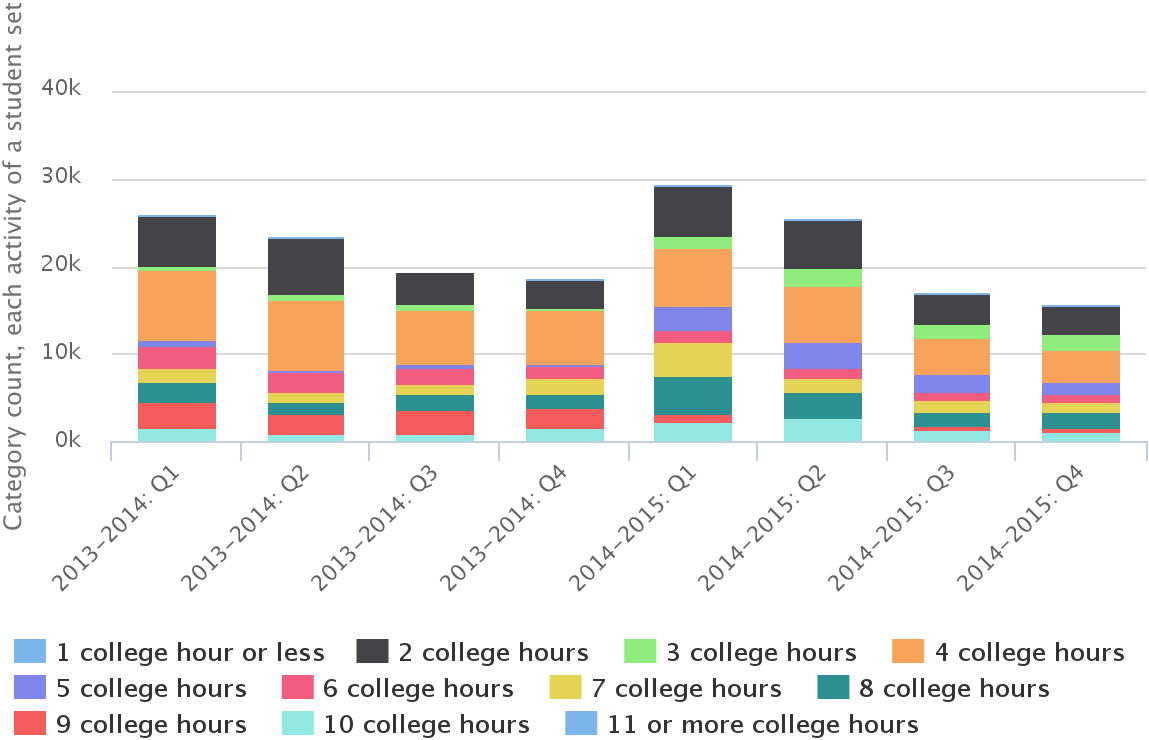
\includegraphics[width=80mm]{dayLengthsStudents.png}
	\caption{Day lengths for students}
	\label{fig:dayLengtsStudents}
\end{figure}

The next statistic is about the wasted hours of teachers and students, which was also in interest by the KPIs. The bar graph in Figure \ref{fig:wastedHours} shows the distribution between useful and 'wasted' hours.

\begin{figure}[!h]
	\centering
	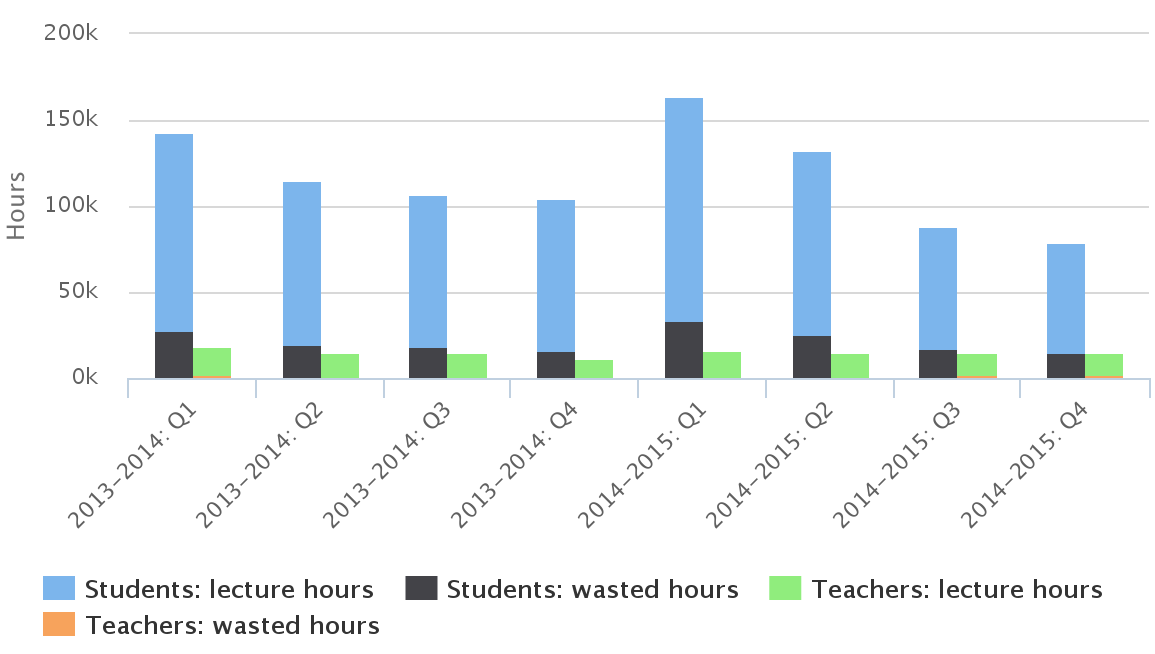
\includegraphics[width=80mm]{wastedHours.png}
	\caption{Wasted hours for students and teachers}
	\label{fig:wastedHours}
\end{figure}

Furthermore we investigated the distribution of lecture types among activities, Figure \ref{fig:lectureTypes} shows the result. For each quartile the number of activities of a certain lecture type can be seen.

\begin{figure}[!h]
	\centering
	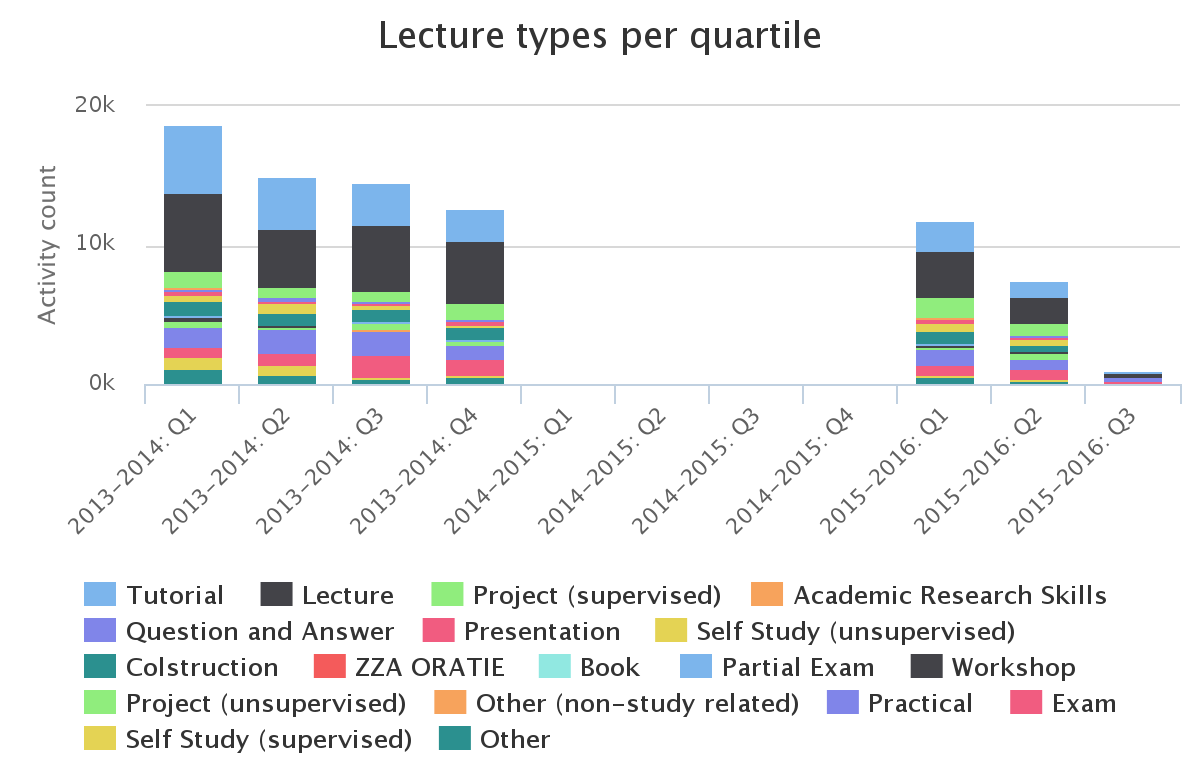
\includegraphics[width=80mm]{lectureTypes.png}
	\caption{Lecture types}
	\label{fig:lectureTypes}
\end{figure}

As last we have counted the number of teachers, student sets and activities per quartile, these could be used to correct the other data or give insight in the activity on the university.

\section{Discussion}
To mention:
\begin{itemize}
	\item Too much data conversion, rather do it once
	\item automating XQuery is hard, but might have saved time	
	\item students assigned to multiple sets, changes statistics
	\item splitting on student sets and teachers changes statistics
	\item teachers are sometimes split by space, we only detect \code{;}
	\item wasted hours: breaks included
	\item rooms used, weird numbers
\end{itemize}

Although results seem quite accurate with such large and inconsistent datasets, results are always skewed. This is certainly not different in our case. The datasets show many inconsistencies which already made the first step of translating the Excel data into an insert query for the database a very complex job. Firstly, many filters needed to be applied to obtain a working insert query. It is possible that some of these filters have altered data in a few cases, however this is quite impossible to validate.

\subsection{Assumptions}
We were given a set of KPIs and questions to perform analyses with on our datasets. However, it was not obvious in all cases how to interpret these. Therefore, we had to make certain assumptions:
\begin{itemize}
	\item We defined a contact hour or college hour as 45 minutes (rather than a clock hour)
	\item We assumed that student sets and teacher were separated with a semicolon
	\item Interpretation of KPI 4 in table \ref{table:kpiAndExploration} on page \pageref{table:kpiAndExploration}: End of last college hour minus start of first college hour is less than 495 minutes (11 college hours).
	\item Interpretation of KPI 6 in table \ref{table:kpiAndExploration} on page \pageref{table:kpiAndExploration}: Evening classes are classes after the 9\textsuperscript{th} (college) hour (after 17:30 or 5.30 PM)
	\item For KPI 9 in table \ref{table:kpiAndExploration} on page \pageref{table:kpiAndExploration}: We defined the total minutes of educational hours as;
	\begin{itemize} 
	\item minutes a day: $9*45=405$ minutes
	\item five days in a week: $5*405=2025$ minutes
	\item 4 quartiles counting ten weeks each (eight weeks of regular education and two exam weeks): $4*10*2025=81000$ minutes
	\end{itemize}
\end{itemize}

\subsection{Corrections}
In order to come up with more or less accurate results we had to perform multiple corrections, namely:
\begin{itemize}
	\item With teachers we discovered that it could occur in some circumstances that a teacher actually had more contact minutes a day then there was between the start of his/hers first activity and last activity. This means that the teacher has overlapping activities in the dataset. In order to correct this, when we observed this behaviour we set it to the actual time between the first and the last activity.
	\item There were many cases in which no date was given. The only possible option for us was to neglect this entry in our results.
	\item Also, in many cases the start and end time were missing, so these entries were not accounted for either.
\end{itemize}

\subsection{Inconsistencies}
\begin{itemize}
	\item It can occur that a student is actually present in multiple student sets. Therefore a student set does not represent an individual student.
	\item It came to our eye that there were some cases in which teachers were separated by a space; this could not be accounted for in the results since it is impossible to build an accurate filter for that.
	\item In the dataset used for analysing the different lecture types, data from 2014 was missing.
\end{itemize}
\section{Conclusion}
To conclude, we have seen that the KPIs set as a target by the University itself are not that well defined and certainly not achieved in most cases. Elaborating on this, the results show that the University at least tries some form of implementing the KPIs in the timetable algorithms. However, we suspect that there are many improvements possible to boost the compliance rates of the KPIs.

Moreover, with more data and specifically more accurate and consistent data, it becomes possible to do a more in-depth analysis on different aspects. For example, it could be interesting to see how the different locations for a particular student are spread out around the campus. With the current data set, this is nearly impossible but when more data is available (possibly a dataset with distances between different locations) this becomes more doable.
\section{Appendices}
\subsection{KPI and Exploration results}
See table \ref{table:kpiAndExploration} on page \pageref{table:kpiAndExploration} of this paper.
\begin{table*}[!h]
	\centering
	\caption{KPI and Exploration results}
	\label{table:kpiAndExploration}
	\begin{tabular}{llll}
		\hline
		\textbf{\#} & \textbf{Key Performance Indicator (KPI)}                                                                                                                                                                                                                                       & \textbf{2013-2014}                                                      & \textbf{2014-2015}                                                    \\ \hline
		1           & Students have a minimum of 4 contact hours on any day                                                                                                                                                                                              & 75.06\%                                                                 & 71.04\%                                                               \\
		2           & Students have a maximum of 6 contact hours on any day                                                                                                                                                                                              & 58.84\%                                                                 & 63.07\%                                                               \\
		3           & Students have a maximum of 2 free hours in 1 series on any day                                                                                                                                                                                     & 81.29\%                                                                 & 70.93\%                                                               \\
		4           & \begin{tabular}[c]{@{}l@{}}The timetable of students have a maximum of 11 college hours on any\\ day. This means 8:15 clock hours, which is the time between start of\\ the first college and the end of the last college on any day)\end{tabular} & 71.69\%                                                                 & 70.44\%                                                               \\
		5           & \begin{tabular}[c]{@{}l@{}}If a student has a class at the 11th and 12th college hour, then that\\ student has no class at the 1st and 2nd college hour the next day\end{tabular}                                                                                                            & Violated 269 times                                                        & Violated 99 times                                                       \\
		6           & At Fridays there are no evening classes                                                                                                                                                                                                            & Violated 232 times                                                        & Violated 255 times                                                      \\
		7           & A teacher has a maximum of 8 contact hours per day                                                                                                                                                                                                 & 94.39\%                                                                 & 93.64\%                                                               \\
		8           & \begin{tabular}[c]{@{}l@{}}If a teacher has a class at the 11th and 12th college hour, then that\\ teacher has no class at the 1st and 2nd college hour the next day\end{tabular}                                                                  & Violated 23 times                                                         & Violated 35 times                                                       \\
		9           & \begin{tabular}[c]{@{}l@{}}Rooms must have an occupation of at least 70\%. Occupation is defined\\ as follows: occupying a space (room) by the timetabling process during\\ educational weeks\end{tabular}                                         & 0.37\% (just one room)                                                  & 0.00\%                                                                \\
		10          & Student set with the most 'wasted' time                                                                                                                                                                                                            & \begin{tabular}[c]{@{}l@{}}ATLAS B1 SEM1 A\\ 10320 minutes\end{tabular} & \begin{tabular}[c]{@{}l@{}}ITC AES-ERE 01\\ 8850 minutes\end{tabular} \\
		11          & Teacher with the most 'wasted' time                                                                                                                                                                                                                & \begin{tabular}[c]{@{}l@{}}WW Wits\\ 10320 minutes\end{tabular}         & \begin{tabular}[c]{@{}l@{}}G Meinsma\\ 7860 minutes\end{tabular}     
	\end{tabular}
\end{table*}
\section{Acknowledgements}
We would like to use this opportunity to thank the University of Twente for kindly sharing the datasets of the past two educational years concerning the timetabling schedules with us. Special thanks to Djoerd Hiemstra and Rudy Oude Vrielink for introducing the topic of XML and timetabling.

\bibliographystyle{ieeetr}
\bibliography{TimeTabling}

\end{document}
